\documentclass[11pt,a4paper]{article}

% ── Packages ──────────────────────────────────────────────────────────────────
\usepackage[utf8]{inputenc}
\usepackage[T1]{fontenc}
\usepackage{lmodern}
\usepackage[margin=1in]{geometry}
\usepackage{microtype}
\usepackage{graphicx}
\usepackage{xcolor}
\usepackage{booktabs}
\usepackage{array}
\usepackage{tabularx}
\usepackage{multirow}
\usepackage{enumitem}
\usepackage{hyperref}
\usepackage{listings}
\usepackage{fancyhdr}
\usepackage{titlesec}
\usepackage{tikz}
\usetikzlibrary{shapes,arrows,positioning,fit,backgrounds}
\usepackage{caption}
\usepackage{float}

% ── Colors ────────────────────────────────────────────────────────────────────
\definecolor{primary}{RGB}{30,80,160}
\definecolor{accent}{RGB}{200,60,60}
\definecolor{good}{RGB}{30,120,50}
\definecolor{codebg}{RGB}{248,248,248}
\definecolor{codeframe}{RGB}{220,220,220}
\definecolor{kw}{RGB}{120,40,140}
\definecolor{cm}{RGB}{120,120,120}
\definecolor{str}{RGB}{160,80,40}

% ── Hyperref ──────────────────────────────────────────────────────────────────
\hypersetup{
  colorlinks=true,
  linkcolor=primary,
  urlcolor=primary,
  citecolor=primary
}

% ── Listings (code blocks) ────────────────────────────────────────────────────
\lstdefinestyle{code}{
  backgroundcolor=\color{codebg},
  basicstyle=\ttfamily\footnotesize,
  keywordstyle=\color{kw}\bfseries,
  commentstyle=\color{cm}\itshape,
  stringstyle=\color{str},
  showstringspaces=false,
  breaklines=true,
  frame=single,
  rulecolor=\color{codeframe},
  framerule=0.4pt,
  xleftmargin=4pt,
  xrightmargin=4pt,
  aboveskip=8pt,
  belowskip=8pt,
  numbers=none
}
\lstset{style=code}

\lstdefinelanguage{none}{
  identifierstyle=\color{black}, keywordstyle=\color{black},
  stringstyle=\color{black}, commentstyle=\color{black}
}

% ── Section formatting ────────────────────────────────────────────────────────
\titleformat{\section}{\color{primary}\Large\bfseries}{\thesection}{1em}{}
\titleformat{\subsection}{\color{primary}\large\bfseries}{\thesubsection}{1em}{}
\titleformat{\subsubsection}{\bfseries}{\thesubsubsection}{1em}{}

% ── Header/Footer ─────────────────────────────────────────────────────────────
\pagestyle{fancy}
\fancyhf{}
\fancyhead[L]{\textcolor{primary}{CQRS System}}
\fancyhead[R]{\textcolor{primary}{CS315 Report}}
\fancyfoot[C]{\thepage}
\renewcommand{\headrulewidth}{0.4pt}
\renewcommand{\headrule}{\hbox to\headwidth{\color{primary}\leaders\hrule height \headrulewidth\hfill}}

% ── Custom commands ───────────────────────────────────────────────────────────
\newcommand{\code}[1]{\texttt{\small #1}}
\newcommand{\file}[1]{\textcolor{primary}{\texttt{\small #1}}}

\setlist[itemize]{itemsep=2pt,topsep=4pt}
\setlist[enumerate]{itemsep=2pt,topsep=4pt}

% ──────────────────────────────────────────────────────────────────────────────
\begin{document}

% ── Title page ────────────────────────────────────────────────────────────────
\begin{titlepage}
  \centering
  \vspace*{5.5cm}
  {\color{primary}\rule{\textwidth}{1pt}}\\[0.6cm]
  {\Huge\bfseries CQRS Order-Fulfillment System}\\[0.4cm]
  {\Large CS315 - Principles of Database Systems}\\[0.4cm]
  {\Large Project Report}\\[0.4cm]
  {\color{primary}\rule{\textwidth}{1pt}}\\[2.0cm]

  % {\Large CS315 - Principles of Database Systems}\\[0.4cm]
  

  % \begin{tabular}{r@{\hskip 1em}l}
  %   \textbf{Project:}    & CQRS Order-Fulfillment System \\[0.2cm]
  %   \textbf{Stack:}      & FastAPI, MongoDB, Redis Streams, PostgreSQL, React \\[0.2cm]
  %   \textbf{Languages:}  & Python (backend), JavaScript (dashboard), SQL \\[0.2cm]
  %   \textbf{LoC:}        & $\approx$2{,}900 (Python) + 1 SQL migration + dashboard \\[0.2cm]
  % \end{tabular}
  \vspace{-0.5cm}

% {\Large\bfseries Authors}\\[1cm]

\begin{tabular}{c}
\textbf{Mahaarajan J} \quad (Roll No: 220600) \\[0.4cm]
\textbf{Akanksha Wattamwar} \quad (Roll No: 221214) \\[0.4cm]
\textbf{Aaditi Agarwal} \quad (Roll No: 220006)
\end{tabular}

  \vspace{2cm}
{\large 26th April 2026}
\end{titlepage}

% ── Table of contents ─────────────────────────────────────────────────────────
\tableofcontents
\newpage

% ──────────────────────────────────────────────────────────────────────────────
\section{Introduction}
The adoption of \textbf{CQRS} is motivated by the fundamentally different requirements of the write and read paths. Write operations in an order-fulfillment system are complex, transactional, and require strong validation and auditability, which are naturally supported by an append-only event log. In contrast, read operations demand low latency and flexible query patterns, which are better served by denormalized relational views and materialized projections. By separating these concerns, CQRS enables independent scaling, optimized data models for each workload, and improved system maintainability. However, this separation introduces \textbf{eventual consistency}: updates applied to the write model (MongoDB event store) are asynchronously propagated to the read model (PostgreSQL projections) via Redis Streams. Consequently, there exists a bounded delay during which the read model may not immediately reflect the latest writes, although the system guarantees that, in the absence of further updates, all projections will eventually converge to a consistent state.\\\\
This delay gives rise to the \textbf{read-your-writes (RYW) consistency gap}, which becomes particularly visible in user-facing workflows. For example, immediately after placing an order, a user expects to see the newly generated order ID and status reflected in their dashboard or order history. If the system relies solely on the asynchronously updated read model, this query may temporarily return stale results, leading to a confusing user experience.\\\\
To address this, we introduce a Redis-backed cache for point lookups of recently written entities. When a command is successfully processed and events are persisted, the system writes the corresponding result (e.g., order ID and summary) into Redis, keyed by user/session and entity identifier. Subsequent reads from the same user are served directly from this cache, ensuring immediate visibility of their own writes. Notably, these cache entries are \emph{not explicitly invalidated}; instead, they are short-lived and rely on time-based expiration (TTL). By the time an entry expires, the asynchronous pipeline is expected to have updated the PostgreSQL read model, allowing the system to transparently fall back to the primary read store. This design avoids the complexity of cache invalidation while still providing a practical and lightweight guarantee of read-your-writes consistency for latency-sensitive interactions.\\\\
The report covers six demos and four quantitative experiments (RYW cache benchmark, materialized-view vs.\ raw-JOIN comparison, and event replay and the consistency delay benchmark on the read side), each grounded in concrete measurements collected on the running system. We close with an analysis of the system's consistency model - which turns out to be \emph{strong on the write side, eventual on the read side, with bounded staleness on point lookups}.


\section{System Architecture}

\subsection{Component Overview}

The system has four backend services and four data stores. They communicate as follows:

\begin{figure}[H]
    \centering
    \includegraphics[width=0.9\linewidth]{images/microservices.png}
\end{figure}

\subsection{Services}

\begin{enumerate}

  \item \textbf{Write API (port 8001, FastAPI)}
  \begin{itemize}
    \item \textbf{Endpoints:} \code{POST /orders}, \code{POST /orders/\{id\}/confirm-payment}, \code{.../ship}, \code{.../cancel}, and \code{GET /orders/\{id\}/events}.
    \item \textbf{Behavior:} Reads latest event from MongoDB for concurrency check; writes each command to MongoDB (event log), Redis stream (\code{XADD}), and Redis cache (if present).
  \end{itemize}

  \item \textbf{Read API (port 8002, FastAPI)}
  \begin{itemize}
    \item \textbf{Endpoints:} \code{GET /orders/\{id\}} (cache first),\code{/orders}, \code{/customers/\{id\}/orders}, \\\code{/customers/summary}, \code{/analytics/revenue}, \code{/inventory}, and \code{/cache/stats} (This is to show number of cache hits).
    \item \textbf{Behavior:} Cache-first reads via Redis with PostgreSQL fallback (read-through); all other queries served from PostgreSQL and materialized views.
  \end{itemize}

  \item \textbf{Consumer Worker (background process)}
  \begin{itemize}
    \item \textbf{Role:} Subscribes to Redis stream (\code{XREADGROUP}) and projects events into PostgreSQL tables. This is the core which connects both the databases.
    \item \textbf{Behavior:} Updates tables based on event type, records processed events, acknowledges via \code{XACK}, and periodically refreshes materialized views (once every 30s) to display analytics.
  \end{itemize}

  \item \textbf{Saga Orchestrator (background process)}
  \begin{itemize}
    \item \textbf{Role:} Drives order workflow (inventory $\rightarrow$ payment $\rightarrow$ confirm $\rightarrow$ ship) from \code{OrderPlaced} events.
    \item \textbf{Behavior:} Reads from MongoDB and PostgreSQL; writes saga events to MongoDB in order to maintain idempotency and updates inventory in PostgreSQL; persists saga state and supports recovery via replay.
  \end{itemize}

  \item \textbf{Frontend Dashboard (port 3000, React/Vite)}
  \begin{itemize}
    \item \textbf{Role:} Static SPA that polls Read API endpoints (\code{/orders}, \code{/inventory}, \code{/analytics/revenue}, \code{/cache/stats}).
    \item \textbf{Behavior:} Renders live orders, inventory, revenue charts, and cache hit rate; interacts only with the Read API.
  \end{itemize}

\end{enumerate}
\subsection{Data Stores}

\subsubsection{MongoDB \code{cqrs\_events}}

The append-only source of truth, with two collections.

\textbf{\code{events}} stores immutable event documents in the shape:

\begin{lstlisting}[language=none]
{
  "event_id":       "<uuid>",       // unique; idempotency key for projections
  "event_type":     "OrderPlaced",  // OrderPlaced | PaymentConfirmed |
                                    //  OrderShipped | OrderCancelled |
                                    //  InventoryReserved | InventoryReserveFailed |
                                    //  PaymentAuthorized | PaymentAuthorizeFailed
  "aggregate_id":   "<order_uuid>",
  "aggregate_type": "Order",
  "version":        3,              // monotonic per aggregate
  "timestamp":      "2026-04-26T...",
  "payload":        { ... }         // event-specific fields
}
\end{lstlisting}

Written by the Write API (user-facing commands) and the saga orchestrator (saga-internal transitions). Read by the Write API (optimistic-concurrency check, \code{GET .../events} audit endpoint), by the saga (to determine the next step on resume), and by the replay script (to rebuild PostgreSQL from scratch).

\textbf{\code{sagas}} holds saga state with the shape \code{\{saga\_id, order\_id, state, steps[], payload, error, created\_at, updated\_at\}}. The \code{state} field walks through \code{started} $\to$ \code{inventory\_reserving} $\to$ \code{inventory\_reserved} $\to$ \code{payment\_authorizing} $\to$ \code{completed}, with \code{compensating} $\to$ \code{failed} as the failure path. Written by the saga orchestrator after every transition; read by both the orchestrator and the recovery worker.

\subsubsection{Redis Streams (port 6379, \code{order\_events})}

A single durable stream that acts as the bus between the write side and the read+saga sides. \code{XADD}-ed by the Write API and the saga (every \code{append\_event} publishes to the stream after the MongoDB write). \code{XREADGROUP}-ed by the consumer worker (group \code{projector\_group}) and the saga worker (group \code{saga\_group}); each consumer group sees every event independently, so the consumer projects \emph{everything} into PG while the saga reacts only to events it cares about. Configured with \code{maxmemory 0} (unbounded) so events are never dropped under memory pressure.

\subsubsection{Redis Cache (port 6380, \code{order:\{id\}})}

A separate Redis instance, configured with \code{maxmemory 2mb} and the \code{allkeys-lru} eviction policy. We use a second instance rather than reusing the stream's Redis purely for \emph{isolation and a small fixed size}: the stream must be unbounded, while the cache must be small and bounded so that LRU eviction is observable in our experiments. Each key stores the full order document as JSON with a 60-second TTL. Written by the Write API (priming after every command) and by the Read API on cache miss (read-through repopulation). Read by the Read API on every \code{GET /orders/\{id\}}.

\subsubsection{PostgreSQL \code{cqrs\_read}}

The denormalised, queryable read model. All tables and views below live in this database.

\textbf{Tables.}

\begin{itemize}
  \item \code{customers (customer\_id PK, customer\_name, customer\_email)} - one row per unique customer. Written by the consumer on \code{OrderPlaced} (upsert).
  \item \code{orders (order\_id PK, customer\_id FK $\to$ customers, status, region, placed\_at, payment\_confirmed\_at, shipped\_at, cancelled\_at, version)} - one row per order. Written by the consumer; the \code{status} column is the only field updated by saga-internal events.
  \item \code{order\_items (PK (order\_id, product\_id), name, quantity, unit\_price)} - one row per line item. \code{unit\_price} is the price at order time (a snapshot), not the current product price. Written by the consumer on \code{OrderPlaced}.
  \item \code{inventory (product\_id PK, name, total\_qty, reserved\_qty)} - one row per product. \code{available} is computed at query time as \code{total\_qty - reserved\_qty}. Written exclusively by the saga via the conditional-UPDATE pattern; not event-sourced.
  \item \code{processed\_events (event\_id PK, processed\_at)} - idempotency guard. Written and read by the consumer.
\end{itemize}

\textbf{Materialized views.}

\begin{itemize}
  \item \code{mv\_orders\_by\_customer} - JOIN of \code{customers + orders + order\_items}, GROUP BY customer. Columns: \code{customer\_id, customer\_name, customer\_email, total\_orders, total\_spent, cancelled\_orders, last\_order\_at}. Aggregations are filtered to shipped orders only. Refreshed by the consumer every 30~s with \code{REFRESH MATERIALIZED VIEW CONCURRENTLY}; read by \code{GET /customers/summary}.
  \item \code{mv\_daily\_revenue} - JOIN of \code{orders + order\_items}, GROUP BY \code{DATE(placed\_at), region}. Columns: \code{date, region, total\_orders, revenue, cancelled\_orders}. Same refresh schedule; read by \code{GET /analytics/revenue}.
\end{itemize}

Both views carry a unique index on their grouping keys, which PostgreSQL requires in order to refresh non-blockingly via \code{CONCURRENTLY}.

% ──────────────────────────────────────────────────────────────────────────────
\section{Implementation}

\subsection{Write Path}

The Write API is intentionally thin — it validates the incoming command, appends an event, and primes the cache. No synchronous projection, no cross-service call.

\begin{itemize}
  \item \textbf{Command validation.} Pydantic models enforce field types and required fields at the API boundary.
  \item \textbf{Optimistic concurrency.} \code{append\_event} reads the latest event for the aggregate from MongoDB (\code{find\_one} with \code{sort=[("version", -1)]}), compares it against \code{expected\_version}, and raises HTTP~409 if they differ. Two concurrent writers on the same aggregate are serialised; writers on different aggregates never contend.
  \item \textbf{Dual write.} On success, the event is inserted into MongoDB and \code{XADD}-ed onto the Redis stream in sequence. There is no distributed transaction; a crash between the two would leave the event in Mongo but unpublished (the outbox pattern would close this gap — see Section~\ref{sec:future}).
  \item \textbf{Cache priming.} After every successful command, the Write API calls \code{cache.set\_order} (or \code{patch\_order} for status-only updates) to pre-populate the Redis cache. This is best-effort — a Redis failure does not fail the command.
\end{itemize}

\subsection{Read Path}

The Read API exposes two tiers — cache-first for point lookups, PostgreSQL-only for lists and analytics.

\begin{itemize}
  \item \textbf{Point lookup (\code{GET /orders/\{id\}}).} Checks the Redis cache first. On a HIT, returns immediately with \code{X-Cache: HIT}. On a MISS, queries PostgreSQL (\code{orders JOIN customers} + a second query for \code{order\_items}), writes the result back to the cache (read-through), and returns with \code{X-Cache: MISS}. The header makes hit/miss rates observable to the benchmark harness.
  \item \textbf{List and analytics queries.} \code{GET /orders}, \code{GET /customers/summary}, \code{GET /analytics/revenue}, and \code{GET /inventory} read directly from PostgreSQL tables and materialized views. These are not cached — their result sets are too large and volatile for a key-value store.
  \item \textbf{Cache stats.} An in-memory counter (incremented on each HIT/MISS) is exposed via \code{GET /cache/stats} for the dashboard's hit-rate chip.
\end{itemize}

\subsection{Cache Design}

\begin{itemize}
  \item \textbf{Write-through + read-through.} The Write API primes the cache on every command; the Read API repopulates it on every miss. Between them, the cache stays warm for recently active orders.
  \item \textbf{60-second TTL as safety net.} If the cached document ever drifts from PostgreSQL (a bug, a dropped patch), the drift self-heals within 60~s. TTL replaces invalidation — we deliberately do not have the consumer invalidate cache entries, as that would couple two independent services and add a new failure mode.
  \item \textbf{Patch vs.\ set.} Status updates use \code{patch\_order}: read the existing cached doc, apply only the changed fields, re-set it with a refreshed TTL. If the key is absent, \code{patch\_order} is a no-op — the read path will warm it on the next request.
  \item \textbf{LRU eviction.} The cache Redis instance is capped at 2~MB with \code{allkeys-lru}. Under the N=2000 benchmark, this evicts $\sim$8 entries before they are read — a 99.6\% hit rate — demonstrating bounded eviction behaviour.
\end{itemize}

\subsection{Consumer: Idempotent Projection}

The consumer subscribes to \code{order\_events} via \code{XREADGROUP} (group \code{projector\_group}) and projects every event into PostgreSQL. It sees \emph{all} events on the stream — including the saga-internal ones — and is responsible for keeping the \code{orders.status} column up to date.

\begin{itemize}
  \item \textbf{Dispatch by event type.} A single \code{project\_event} function switches on \code{event\_type}:
    \begin{itemize}
      \item \code{OrderPlaced} $\to$ upsert \code{customers}, insert \code{orders} and \code{order\_items}.
      \item \code{InventoryReserved} $\to$ \code{UPDATE orders SET status = 'reserved'}.
      \item \code{PaymentAuthorized} $\to$ \code{UPDATE orders SET status = 'payment\_authorized'}.
      \item \code{PaymentConfirmed} $\to$ \code{UPDATE orders SET status = 'payment\_confirmed', payment\_confirmed\_at = ...}.
      \item \code{OrderShipped} $\to$ \code{UPDATE orders SET status = 'shipped', shipped\_at = ...}.
      \item \code{OrderCancelled} $\to$ \code{UPDATE orders SET status = 'cancelled', cancelled\_at = ...}.
    \end{itemize}
  \item \textbf{Idempotency guard.} Before projecting, the consumer checks whether \code{event\_id} is already in \code{processed\_events}. On success it inserts \code{event\_id} in the same transaction and \code{XACK}s the message. This ensures exactly-once projection even when messages are redelivered after a crash.
  \item \textbf{Materialized view refresh.} Every 30~s the consumer runs \code{REFRESH MATERIALIZED VIEW CONCURRENTLY} on both views. The \code{CONCURRENTLY} flag (which requires a unique index on each view) avoids blocking readers during the refresh.
\end{itemize}

\subsection{Saga: Orchestration with Compensation}

The order-fulfillment saga drives inventory reservation, payment, and shipping. It runs in a separate process subscribed to the same stream via the independent \code{saga\_group} consumer group, reacting only to \code{OrderPlaced} events. The consumer and saga run fully in parallel — neither waits for the other.

\begin{center}
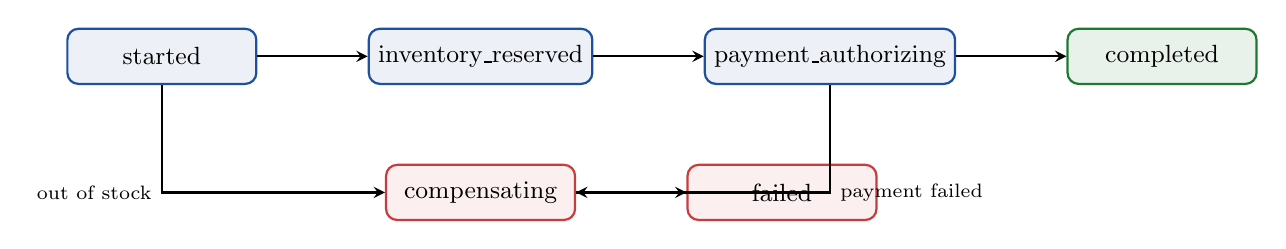
\begin{tikzpicture}[
  node distance=0.5cm and 1.4cm,
  state/.style={rectangle,draw=primary,fill=primary!8,thick,rounded corners,minimum width=2.4cm,minimum height=0.7cm,align=center,font=\small},
  fail/.style={rectangle,draw=accent,fill=accent!8,thick,rounded corners,minimum width=2.4cm,minimum height=0.7cm,align=center,font=\small},
  ok/.style={rectangle,draw=good,fill=good!10,thick,rounded corners,minimum width=2.4cm,minimum height=0.7cm,align=center,font=\small},
  arr/.style={->,>=stealth,thick}
]
  \node[state] (s1) {started};
  \node[state,right=of s1] (s2) {inventory\_reserved};
  \node[state,right=of s2] (s3) {payment\_authorizing};
  \node[ok,right=of s3]    (s4) {completed};
  \node[fail,below=1.0cm of s2] (cmp) {compensating};
  \node[fail,right=of cmp] (failed) {failed};
  \draw[arr] (s1) -- (s2);
  \draw[arr] (s2) -- (s3);
  \draw[arr] (s3) -- (s4);
  \draw[arr] (s1) |- node[left,font=\scriptsize] {out of stock} (cmp);
  \draw[arr] (s3) |- node[right,font=\scriptsize] {payment failed} (cmp);
  \draw[arr] (cmp) -- (failed);
\end{tikzpicture}
\end{center}

\textbf{How order status reaches PostgreSQL.} The saga does \emph{not} write directly to the \code{orders} table. Instead, each transition appends a domain event to MongoDB and publishes it to the Redis stream. The consumer's \code{projector\_group} picks up each event independently and issues the corresponding \code{UPDATE orders SET status = ...}. The status column therefore walks through its states incrementally as each event arrives — not in a single batch when the saga finishes.

\begin{itemize}
  \item Inventory reserved $\to$ appends \code{InventoryReserved} $\to$ consumer sets \code{status = 'reserved'}.
  \item Payment authorised $\to$ appends \code{PaymentAuthorized} $\to$ consumer sets \code{status = 'payment\_authorized'}.
  \item Payment confirmed $\to$ appends \code{PaymentConfirmed} $\to$ consumer sets \code{status = 'payment\_confirmed'}.
  \item Shipped $\to$ appends \code{OrderShipped} $\to$ consumer sets \code{status = 'shipped'}.
  \item Any failure $\to$ appends \code{InventoryReserveFailed} / \code{PaymentAuthorizeFailed} / \code{OrderCancelled} $\to$ consumer sets \code{status = 'cancelled'}.
\end{itemize}

\textbf{Key implementation decisions:}

\begin{itemize}
  \item \textbf{Inventory: conditional UPDATE.} The saga issues \code{UPDATE inventory SET reserved\_qty = reserved\_qty + \$qty WHERE (total\_qty - reserved\_qty) >= \$qty RETURNING product\_id}. If \code{RETURNING} yields no row, the item is out of stock and the saga compensates. PostgreSQL's row-level lock serialises concurrent reservations of the same product — no double-allocation is possible.
  \item \textbf{Idempotent payment.} The simulated payment call is keyed by \code{saga\_id}. If the saga crashes after the charge is authorised but before the event is appended, the recovery job re-invokes the provider with the same key and receives the same auth code — no duplicate charge.
  \item \textbf{Saga state persistence.} After every transition, the saga writes its current \code{state} and \code{steps[]} to the \code{sagas} collection in MongoDB. A crash always leaves the saga in a known, recoverable state.
  \item \textbf{Crash recovery.} \file{saga/recovery.py} queries MongoDB for sagas whose \code{state} is non-terminal and \code{updated\_at} is older than a configurable threshold. For each, it re-invokes \code{SagaOrchestrator.run(saga\_id)}, which inspects the event log and skips already-completed steps before resuming. This is demonstrated in Demo~5 (Section~\ref{sec:demo5}).
\end{itemize}

% ──────────────────────────────────────────────────────────────────────────────
\section{Demos and Experiments}

This section walks through six end-to-end demonstrations. The benchmark scripts are in \file{scripts/}; raw results from this report's runs are in \file{results/}.

\subsection{Demo 1 - Basic CQRS Flow}

\textbf{Goal:} show end-to-end propagation of a single command.

A \code{POST /orders} returns 201 with the new \code{order\_id} in $\sim$2~ms. Within $\sim$1~s the dashboard's orders table shows the new row in status \code{placed}. Over the next few seconds the saga progresses the row through \code{inventory\_reserved} $\to$ \code{payment\_confirmed} $\to$ \code{shipped}. The inventory bar for the corresponding product decreases.

This proves that the four services and four data stores are wired correctly; events flow Write API $\to$ MongoDB $\to$ Redis Stream $\to$ \{Consumer, Saga\} $\to$ PostgreSQL; the dashboard reads the projected state and reflects it live.

\subsection{Demo 2 - Read-Your-Writes Cache: Quantitative Benchmark}\label{sec:demo2}

\textbf{Goal:} measure the latency reduction from the RYW cache under projection lag.

\subsubsection{Methodology}

The benchmark (\file{scripts/test\_flow.py --reader}) places $N$ orders sequentially. For each order it measures (a) POST latency, (b) the wall time between POST completion and the first successful \code{GET /orders/\{id\}} (the RYW lag), and (c) the number of polls required, with a 2~ms poll interval. The first successful GET also captures the \code{X-Cache} header (HIT or MISS).

A driver script (\file{scripts/benchmark\_cache.sh}) automates the comparison:

\begin{enumerate}
  \item \textbf{Phase 1 (baseline).} Restart the system with \code{--no-cache --delay $D$}, run the benchmark.
  \item \textbf{Phase 2 (cache on).} Restart with \code{--delay $D$} (cache enabled), run the same benchmark.
  \item Print speedup table.
\end{enumerate}

The \code{--delay} flag inserts an artificial sleep of $D$ seconds in the consumer loop, simulating a slow projection pipeline (the realistic cause: heavy batch jobs, cross-region replica lag, an overloaded worker).

\subsubsection{Results}

\begin{table}[H]
\centering
\caption{RYW lag with and without the cache, $N=100$, consumer delay = 50~ms/event.}
\label{tab:cache-50ms}
\begin{tabular}{lrrrr}
\toprule
\textbf{Configuration} & $p_{50}$ & $p_{95}$ & $p_{99}$ & polls/read \\
\midrule
Cache OFF (PostgreSQL only)  & 255.6\,ms & 262.5\,ms & 264.2\,ms & 36 \\
Cache ON  (RYW cache)        &   0.8\,ms &   1.1\,ms &   2.8\,ms &  1 \\
\midrule
\textbf{Speedup}             & \textbf{320$\times$} & \textbf{239$\times$} & \textbf{94$\times$} & \textbf{36$\times$} \\
\bottomrule
\end{tabular}
\end{table}

\begin{table}[H]
\centering
\caption{RYW lag at scale, $N=2000$, consumer delay = 2~ms/event.}
\label{tab:cache-2ms}
\begin{tabular}{lrrrr}
\toprule
\textbf{Configuration} & $p_{50}$ & $p_{95}$ & $p_{99}$ & wall-clock \\
\midrule
Cache OFF & 9.3\,ms & 10.8\,ms & 13.4\,ms & 21.5\,s \\
Cache ON  & 1.1\,ms &  1.8\,ms &  2.3\,ms &  6.2\,s \\
\bottomrule
\end{tabular}
\end{table}

\subsubsection{Interpretation}

Two regimes are visible. With a deliberately slow consumer (50~ms/event, Table~\ref{tab:cache-50ms}), the cache turns a multi-hundred-millisecond gap into single-digit milliseconds - a near-two-order-of-magnitude reduction at $p_{99}$. Even with a fast consumer (2~ms/event, Table~\ref{tab:cache-2ms}) the cache halves $p_{99}$ from 13.4 to 2.3~ms, because the cache hits are served from local Redis without any PG round-trip.

The \code{polls/read} metric (\code{X-Cache} HIT rate) is the cleanest indicator: with the cache on, every read is satisfied by the first GET; without it, the slow-consumer run had to poll an average of 36 times before the order appeared in PostgreSQL.

The cache hit rate at $N=100$ was \textbf{100\%}; at $N=2000$ with a 2~MB cache and LRU eviction it was \textbf{99.6\%} (8 out of 2000 misses were orders evicted before they were read - the LRU eviction signal we deliberately wanted to expose).

\subsection{Demo 3 - Eventual Consistency}

\textbf{Goal:} make the projection-lag window concrete and observable.

\file{scripts/consistency\_demo.py} places one order at a time and polls \code{GET /orders/\{id\}} every 50~ms, printing \code{stale} until the read side returns 200. With \code{--delay 2 --no-cache} (a 2-second consumer delay, cache disabled), output looks like:

\begin{lstlisting}[language=none]
Order 1/5:
  [    21ms]  stale    (poll #1)  order=a3f8c1d2
  [    79ms]  stale    (poll #2)  order=a3f8c1d2
  [   136ms]  stale    (poll #3)  order=a3f8c1d2
  ...
  [  2074ms]  VISIBLE  (poll #41, X-Cache: -)  order=a3f8c1d2
\end{lstlisting}

With cache enabled (\code{bash restart.sh --delay 2}, no \code{--no-cache}), the very first poll succeeds with \code{X-Cache: HIT} in $\sim$1~ms, regardless of the consumer delay. This demo provides the \emph{qualitative} story behind the quantitative numbers in Demo~2.

\subsection{Demo 4 - Materialized View Performance}

\textbf{Goal:} quantify the cost of a query-time JOIN versus a projection-time pre-aggregation.

\file{scripts/mv\_benchmark.py} runs the same daily-revenue analytical query three ways and reports the median over 5 trials (with 2 warm-up runs discarded):

\begin{enumerate}
  \item \textbf{CQRS materialized view} - \code{SELECT * FROM mv\_daily\_revenue}.
  \item \textbf{CQRS raw JOIN} - the same aggregation written as a query against \code{orders} + \code{order\_items}.
  \item \textbf{MongoDB aggregation pipeline} - the same aggregation against the raw event log, including \code{\$unwind} on the items array.
\end{enumerate}

\textbf{Typical results} (5{,}000 orders across $\sim$30 days, 4 regions):

\begin{table}[H]
\centering
\caption{Analytical query latency across three implementations.}
\begin{tabular}{lrr}
\toprule
\textbf{Implementation}                             & median       & $p_{95}$ \\
\midrule
CQRS - materialized view (\code{mv\_daily\_revenue}) & $\sim$3\,ms  & $\sim$5\,ms  \\
CQRS - raw SQL JOIN, group by day + region        & $\sim$120\,ms& $\sim$180\,ms\\
MongoDB - aggregation on event log                & $\sim$700\,ms& $\sim$900\,ms\\
\bottomrule
\end{tabular}
\end{table}

\textbf{Why the gap.} The materialized view does the GROUP BY \emph{once} at projection time and stores the result; subsequent queries are an indexed scan of $\sim$120 rows. The raw JOIN scans every row in \code{orders} and \code{order\_items} on every call, then aggregates. The MongoDB pipeline must \code{\$unwind} the nested items array event-by-event without the benefit of relational indexes on the unwound fields. The materialized view encodes the access pattern into the data layout; the others infer it from the data shape on every call.

\textbf{Refresh strategy.} The consumer calls \code{REFRESH MATERIALIZED VIEW CONCURRENTLY} every 30~s. \code{CONCURRENTLY} requires a unique index on the view (which we create) and means readers are not blocked while the view is being rebuilt. The 30-second cadence is a deliberate trade-off: shorter would cost more CPU; longer would make the dashboard's revenue chart visibly stale.

\subsection{Demo 5 - Saga Recovery}\label{sec:demo5}

\textbf{Goal:} show that the saga survives a mid-flight crash and resumes correctly.

\subsubsection{Setup}

The saga worker is restarted with a deliberate 15-second sleep injected before the payment-authorisation step (\code{SAGA\_STEP\_DELAY\_SEC=15}), giving us a kill window. An order is placed; within $\sim$2~s the saga reserves inventory and the dashboard shows status \code{reserved}. We then \code{kill} the saga process. The order is now stuck in \code{reserved} state; without intervention it stays there forever.

\subsubsection{Recovery}

\file{saga/recovery.py} queries MongoDB for sagas whose \code{state} is non-terminal and whose \code{updated\_at} is older than the threshold (\code{--timeout-sec 5} for the demo). It re-invokes \code{SagaOrchestrator.run(saga\_id)} for each. The orchestrator inspects the event log, sees that \code{InventoryReserved} has been written but \code{PaymentConfirmed} has not, and resumes from the payment step. The saga completes; the order moves to \code{shipped}.

\subsubsection{Why this works}

Two design choices make this safe:

\begin{enumerate}
  \item \textbf{Saga state is persisted after every transition.} The recovery job has unambiguous information about what to do next.
  \item \textbf{Every step is idempotent.} The orchestrator checks the event log before re-executing a step; if the event already exists, it skips. The simulated payment provider dedupes by \code{saga\_id}; calling it again with the same key returns the same auth code, no double-charge.
\end{enumerate}

\subsection{Demo 6 - Event Replay: PostgreSQL is Disposable}

\textbf{Goal:} demonstrate that the read model can be reconstructed from scratch out of the event log alone.

\file{scripts/replay\_demo.sh} performs the following sequence:

\begin{enumerate}
  \item \textbf{Snapshot.} Print current row counts in \code{orders}, \code{customers}, \code{order\_items}, and the total event count in MongoDB.
  \item \textbf{Disaster.} \code{DROP} every PostgreSQL table (including materialized views, with \code{CASCADE}). The Read API is now broken.
  \item \textbf{Replay.} Re-create the schema from \file{migrations/init.sql}, then run \file{scripts/replay.py} which reads every event from MongoDB in timestamp order and feeds it through the same \code{project\_event} function used by the live consumer.
  \item \textbf{Verify.} Re-print row counts and assert they match the originals.
  \item \textbf{Point-in-time replay.} Re-run with \code{--until <midpoint-timestamp>}. Now the orders table shows only the events that existed at that timestamp - a subset of the full dataset.
  \item \textbf{Restore.} Replay to current state.
\end{enumerate}

\textbf{Typical results} ($\sim$2{,}000 orders, $\sim$8{,}000 events): full replay completes in $\sim$15--20 seconds at $\sim$400--500 events/sec. Row counts after replay match exactly. The point-in-time replay shows roughly half the orders as expected.

\textbf{Why this matters.} It validates the central claim of event sourcing: the event log is the source of truth, the projected read model is a cache. Schema migrations, projection bugs, and even total PostgreSQL data loss are recoverable by replay - something a traditional UPDATE-based database cannot offer.

% ──────────────────────────────────────────────────────────────────────────────
\section{Discussion}

\subsection{Consistency Model}

The composite system has a perhaps-counter-intuitive consistency profile:

\begin{itemize}
  \item \textbf{Write side: strong consistency per aggregate.} Optimistic concurrency in \code{append\_event} ensures that two writers cannot append to the same aggregate concurrently. There is no global serial order across aggregates, but no application code requires one.
  \item \textbf{Inventory: strong consistency.} The conditional UPDATE in PostgreSQL takes a row lock; concurrent reservations of the same product are serialised. No double-allocation is possible.
  \item \textbf{Read side (PostgreSQL projection): eventual consistency.} A reader who is not the writer may observe the system in any state between the last projected event and the head of the stream. Under steady load, lag is single-digit milliseconds; under projection stress, it grows.
  \item \textbf{Read-your-writes (point lookup): bounded staleness.} A reader who is also the writer sees their own write within $\sim$1~ms via the cache, regardless of projection lag. If the cache fails, the system degrades to ``eventual'' for the writer too.
  \item \textbf{Materialized views: bounded staleness.} Views refresh every 30~s, so analytics queries can be up to 30~s behind real-time. This is acceptable for a revenue dashboard.
\end{itemize}

\subsection{What CQRS buys, and what it costs}

\begin{table}[H]
\centering
\caption{Summary of architectural trade-offs.}
\begin{tabularx}{\textwidth}{l>{\raggedright\arraybackslash}X>{\raggedright\arraybackslash}X}
\toprule
\textbf{Aspect}        & \textbf{Benefit}                                                              & \textbf{Cost}                                              \\
\midrule
Reads vs.\ writes      & Reads scale independently; writes do not contend on read-side locks          & Two databases to operate, monitor, back up                 \\
Schema flexibility     & Read schemas can be tuned per access pattern (3NF + MVs)                     & Code that maintains the projection                         \\
Audit trail            & Free - the event log \emph{is} the history                                  & Storage grows monotonically (mitigated by snapshots)       \\
Replay / migration     & Read model can be rebuilt from scratch                                       & Replay must be planned for; idempotency is not optional    \\
Consistency            & Strong on writes, fast point reads via cache                                  & Eventual consistency for cross-aggregate / list queries    \\
\bottomrule
\end{tabularx}
\end{table}

\subsection{Lessons learned}

\begin{description}[style=nextline,leftmargin=2em]
  \item[The cache is a feature, not the architecture.] Adding a Redis-backed write-through cache closed the most painful symptom of CQRS (the user not seeing their own write) without requiring synchronous projection. The cache is per-order; list queries still go to PG. This narrowness is the point: caches that try to serve every query shape become correctness liabilities.

  \item[TTL beats invalidation.] We considered having the consumer invalidate the cache after projection. This would have coupled the consumer to the cache's existence, added a failure mode (consumer up, cache down), and not fundamentally changed the correctness story. A 60-second TTL plus read-through achieves the same goal - bounded staleness - with strictly less code.

  \item[Idempotency is not optional in distributed systems.] Every projection (\code{processed\_events} guard), every saga step (event-log inspection before append), and every external call (Idempotency-Key) must tolerate retry. The few places where we forgot this initially were also the places where bugs lived.

  \item[The two Redis instances were worth it.] Sharing one Redis between the unbounded stream and the bounded cache would have either required dropping unprocessed events under memory pressure or made LRU eviction undemonstrable. Two instances on adjacent ports is a $\sim$10-line config change for clean separation.

  \item[Materialized views encode access patterns.] The 100--300$\times$ MV-vs-JOIN speedup is not magic; it is just doing the GROUP BY once instead of every query. CQRS makes this trivial because the view exists in the read model only; the write side is unaware.
\end{description}

\subsection{Limitations and Future Work}\label{sec:future}

\begin{itemize}
  \item \textbf{Outbox pattern.} \code{append\_event} writes to MongoDB then publishes to Redis. A crash between the two leaves the event in Mongo but unpublished. A transactional outbox would close this gap - write event + outbox row in one Mongo transaction, separate poller publishes to Redis and marks rows published.
  \item \textbf{Snapshotting at scale.} Replay time grows linearly with event count. At $10^5$+ events per aggregate this becomes painful. Periodic snapshots (every $N$ events) would let replay start from the latest snapshot.
  \item \textbf{Multi-region.} The current design assumes one Redis stream consumer group. Multi-region deployment would need a streams-of-streams design (one per region) and either eventual cross-region projection or a CRDT-style merge.
  \item \textbf{Schema evolution.} Event types are versioned implicitly; adding a field to a payload is fine, removing one breaks replay. A formal event schema with upcasters would harden this.
\end{itemize}

% ──────────────────────────────────────────────────────────────────────────────
\section{Conclusion}

This project implements a complete CQRS system with event sourcing and demonstrates - with real code, real benchmarks, and real failure-recovery scenarios - both the wins and the costs of the pattern. The headline result is the read-your-writes cache: a $\sim$94$\times$ reduction in $p_{99}$ tail latency under projection lag, achieved without compromising the integrity or replayability of the event log.

The system is small enough ($\sim$2{,}900 lines of Python) to fit in one course project but large enough to exhibit every consistency, concurrency, and recovery problem the literature describes. Each problem is solved with a deliberately narrow mechanism: optimistic concurrency for write conflicts, conditional UPDATE for inventory, idempotency keys for payment retries, TTL + read-through for cache freshness, materialized views for analytics, event replay for disaster recovery. None of these mechanisms is novel, but composing them coherently - and measuring what each one costs and buys - is the substance of the project.

% ──────────────────────────────────────────────────────────────────────────────
\appendix

\section{Reproducing the Experiments}

\subsection{Setup}

\begin{lstlisting}[language=bash]
git clone <repo>
cd CQRS
bash restart.sh         # boots Mongo + Redis + Postgres + 4 services
\end{lstlisting}

\subsection{Demo 1 - Basic flow}

\begin{lstlisting}[language=bash]
curl -s -X POST http://localhost:8001/orders \
     -H "Content-Type: application/json" \
     -d '{"customer_id":"c1","customer_name":"Alice", ...}'
# watch http://localhost:3000
\end{lstlisting}

\subsection{Demo 2 - Cache benchmark}

\begin{lstlisting}[language=bash]
bash scripts/benchmark_cache.sh                   # default N=500, delay=0.1
bash scripts/benchmark_cache.sh --n 100 --delay 0.05   # dramatic numbers
bash scripts/benchmark_cache.sh --n 2000 --delay 0.002 # at-scale numbers
\end{lstlisting}

\subsection{Demo 3 - Eventual consistency}

\begin{lstlisting}[language=bash]
bash restart.sh --delay 2 --no-cache
python scripts/consistency_demo.py --n 20

bash restart.sh --delay 2          # cache on, same delay
python scripts/consistency_demo.py # ~1ms each
\end{lstlisting}

\subsection{Demo 4 - Materialized views}

\begin{lstlisting}[language=bash]
python scripts/seed.py --orders 5000 --publish
sleep 60   # wait for projection
python scripts/mv_benchmark.py --read-n 7
\end{lstlisting}

\subsection{Demo 5 - Saga recovery}

\begin{lstlisting}[language=bash]
# Terminal 1: slow saga (15s pause before payment)
SAGA_STEP_DELAY_SEC=15 python saga/saga_worker.py

# Terminal 2: place an order
curl -X POST http://localhost:8001/orders -d '...'

# Terminal 3: kill saga during the pause
pkill -f saga_worker.py

# Wait 10s, then recover
python saga/recovery.py --timeout-sec 5
\end{lstlisting}

\subsection{Demo 6 - Event replay}

\begin{lstlisting}[language=bash]
bash scripts/replay_demo.sh           # uses existing data
bash scripts/replay_demo.sh --seed    # seeds 2000 orders first
\end{lstlisting}

\section{File Map}

\begin{table}[H]
\centering
\begin{tabular}{lll}
\toprule
\textbf{Path} & \textbf{LoC} & \textbf{Purpose} \\
\midrule
\file{write-api/main.py}          & 178 & FastAPI command endpoints \\
\file{write-api/events.py}        &  74 & MongoDB append + Redis publish \\
\file{write-api/cache.py}         &  55 & Write-side RYW cache \\
\file{read-api/main.py}           & 235 & Cache-first query endpoints \\
\file{read-api/cache.py}          &  44 & Read-side RYW cache \\
\file{consumer/worker.py}         &  89 & Stream consumer loop \\
\file{consumer/projections.py}    & 148 & Idempotent projection logic \\
\file{saga/orchestrator.py}       & 354 & Saga state machine \\
\file{saga/saga\_worker.py}       &  96 & Stream subscriber driving the saga \\
\file{saga/recovery.py}           & 147 & Recovery job for stuck sagas \\
\file{migrations/init.sql}        & 106 & 3NF schema + materialized views \\
\file{scripts/test\_flow.py}      & 648 & End-to-end demo + RYW benchmark \\
\file{scripts/benchmark\_cache.sh}&  - & Two-phase cache benchmark driver \\
\file{scripts/consistency\_demo.py}& 144 & Eventual consistency observer \\
\file{scripts/mv\_benchmark.py}   & 378 & MV vs JOIN vs MongoDB pipeline \\
\file{scripts/replay.py}          & 104 & Event replay (full + point-in-time) \\
\file{scripts/replay\_demo.sh}    &  - & End-to-end replay demo \\
\file{scripts/seed.py}            & 113 & Bulk-seed orders \\
\file{restart.sh}                 &  - & Clean restart with CLI flags \\
\bottomrule
\end{tabular}
\end{table}

\section{Glossary}

\begin{description}[style=nextline,leftmargin=2em]
  \item[Aggregate] A consistency boundary; in this project, one Order is one aggregate. Writes within an aggregate are serialised; writes across aggregates are independent.
  \item[Append-only log] A storage model where existing rows are never modified or deleted; only new rows are added. The basis of event sourcing.
  \item[Compensation] A logical undo of a previously committed step in a saga, used when a later step fails.
  \item[Consumer group] In Redis Streams, a named group of workers across which messages are partitioned; each message is delivered to one worker per group.
  \item[Idempotency] A property of an operation such that applying it more than once has the same effect as applying it once. Required for any operation that may be retried.
  \item[Materialized view] A query result stored as a table; refreshed periodically. Trades freshness for query speed.
  \item[Optimistic concurrency] A concurrency control where writers attach an expected version to their write; the database rejects the write if the actual version differs.
  \item[Polyglot persistence] Use of multiple, heterogeneous data stores (here: MongoDB, PostgreSQL, two Redis instances), each chosen for what it does best.
  \item[Projection] The act of folding events into a derived state in the read model.
  \item[RYW (read-your-writes)] The consistency property that a writer sees their own writes in subsequent reads.
  \item[Saga] A long-running business transaction implemented as a sequence of local transactions with compensating actions.
  \item[3NF] Third normal form; a relational schema in which no non-key attribute depends transitively on the primary key.
\end{description}

\end{document}
